
\section{Yearly Average Temperatures in Falsterbo, 1967-2017}
With the release of the International Panel on Climate Change (IPCC)'s Sixth Assessment Report\cite{IPCC} in August 2021 having further highlighted the global increase in average temperatures the topic has once again returned to the forefront of public discourse. The global increase in average temperatures is hardly a novel line of inquiry, however the analysis of temperature trends locally may still be of interest (particularly to those local to the area in question). The data analysed for this section was measured at a measuring station located in Falsterbo in southwestern Skåne, at a height of 1.541m above sea level, at coordinates (in decimal degrees) 55.3837 latitude, 12.8167 longitude.


The data was provided in CSV-format as part of a SMHI-dataset, and analysed using a custom C++ function and plotted using ROOT. The data was handled using line-by-line reading of the data and slicing into strings, slicing the date and temperature in separate strings, the former being used to further create a substring consisting only of the year. This substring is then converted to an integer and used to check first whether the data in question belongs to the relevant range of years. The entire date string is then checked to see wheter or not the data for a new day is being parsed, if not the temperature data is added to a sum and a count of the number of entries for a specific day increased by one, and if yes, the same actions are performed after first taking the average of the sum, pushing it to a vector containing the daily average temperatures of a whole year and zeroing the sum and entry counter. A similar process is used whenever a new year is being iterated upon, in which case the average of the vector containing the daily averages is calculated using a small utility function which loops over all elements, after which it is stored in both a separate vector and in a TGraph object. This is repeated for all lines containing years in the specified range, after which the rest of the lines are just read and then a graph of the data is then plotted from the TGraph object. Worth noting is that the code is unable to account for the quality of the data (in the data set indicated by a G, for controlled and accepted values, and Y for suspect or aggregated values, from roughly checked archive data or real-time data.), nor detect or account missing data.

\begin{figure}[H]
    \centering
    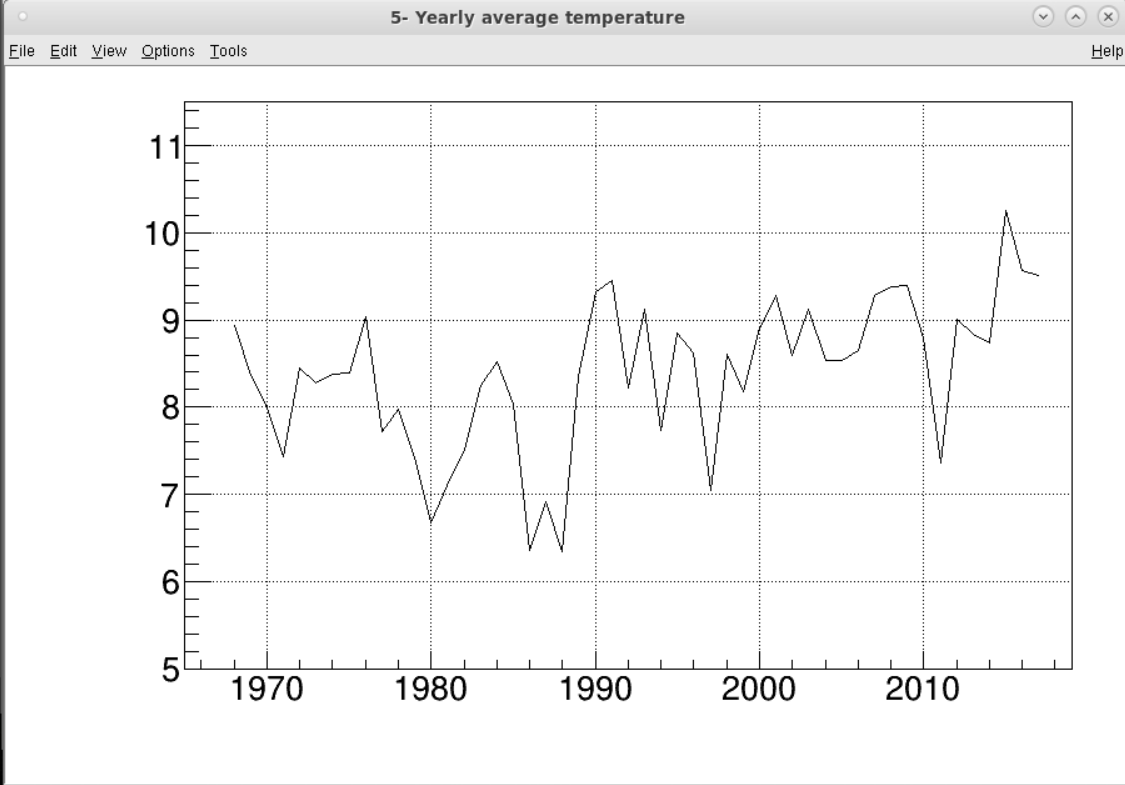
\includegraphics[scale=0.65]{Graph5c.PNG}
    \caption{The yearly average temperatures measured at Falsterbo during 1967-2017.}
    \label{dipole}
\end{figure}

Although no explicit trendline was plotted, the resulting graph still shows a clear upwards trend in temperatures over the period, shifting both high and low peaks towards higher temperatures, which is as expected considering global trends. An abnormaly cold period in the latter half of the 1980's (1986-1988) was noted, although there's no direct indication that this is due to not accounting for missing data or other shortcoming of the code, however the possibility cannot be dismissed.


\section{Refrences}
\begin{thebibliography}{}

\bibitem{IPCC} IPCC, \textit{Climate Change 2021 The Physical Science Basis, Working Group I contribution to the Sixth Assessment Report of the Intergovernmental Panel on Climate Change}

\end{thebibliography}